\documentclass[tikz, border=10pt]{standalone}
\usepackage{tikz}
\usetikzlibrary{positioning, fit, arrows.meta, backgrounds, calc, shapes.geometric, shadows}
\begin{document}

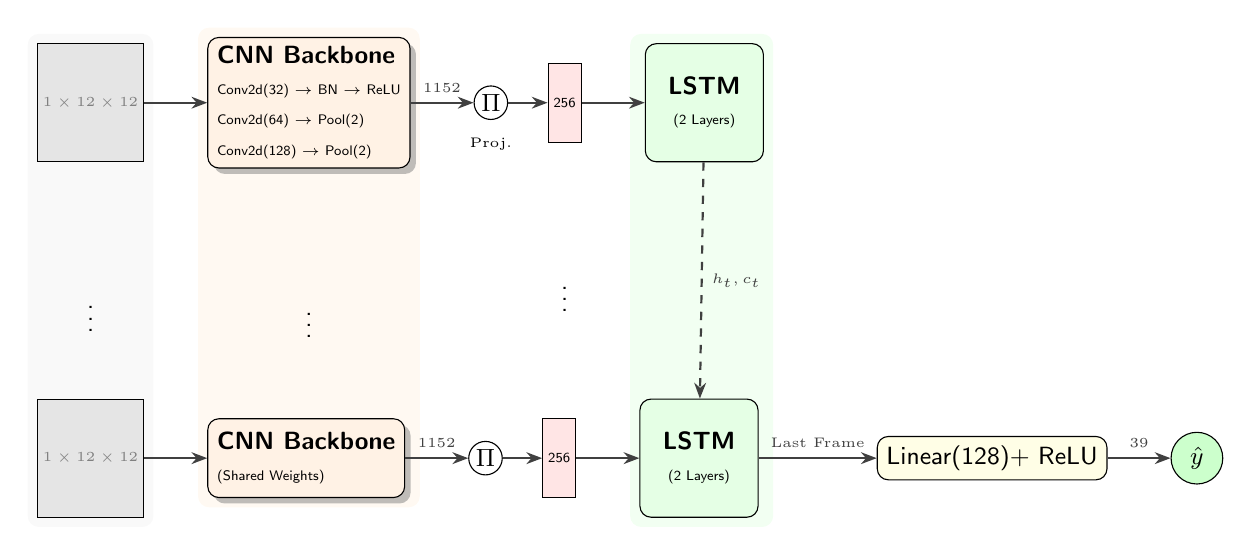
\begin{tikzpicture}[
    font=\sffamily\small,
    >={Stealth[length=2mm]},
    % Styles
    tensor/.style={
        draw, fill=blue!10, rectangle, minimum height=1.5cm, minimum width=0.5cm, align=center, inner sep=2pt
    },
    convblock/.style={
        draw, fill=orange!10, rectangle, rounded corners, minimum height=1cm, minimum width=2.5cm, align=center, drop shadow
    },
    lstm/.style={
        draw, fill=green!10, rectangle, rounded corners, minimum height=1.5cm, minimum width=1.5cm, align=center
    },
    dense/.style={
        draw, fill=purple!10, trapezium, trapezium left angle=70, trapezium right angle=110, minimum height=1cm, align=center
    },
    arrow/.style={->, thick, darkgray},
    label/.style={font=\footnotesize\color{gray}}
]

    % --- TIME STEP 1 ---
    % Input Frame 1
    \node[tensor, fill=gray!20, label=above:{$x_{t_1}$}] (in1) at (0,0) {\tiny $1\times12\times12$};
    
    % CNN Block 1 (Shared)
    \node[convblock, right=0.8cm of in1, align=left] (cnn1) {
        \textbf{CNN Backbone}\\
        \tiny Conv2d(32) $\to$ BN $\to$ ReLU\\
        \tiny Conv2d(64) $\to$ Pool(2)\\
        \tiny Conv2d(128) $\to$ Pool(2)
    };
    
    % Flatten & Project
    \node[right=0.8cm of cnn1] (flat1) [draw, circle, inner sep=1pt, fill=white] {$\Pi$};
    \node[below=0.1cm of flat1, font=\tiny] {Proj.};

    % Feature Vector 1
    \node[tensor, right=0.5cm of flat1, fill=red!10, minimum height=1cm, minimum width=0.3cm] (feat1) {\tiny 256};
    
    % LSTM Cell 1
    \node[lstm, right=0.8cm of feat1] (lstm1) {\textbf{LSTM}\\ \tiny (2 Layers)};

    % --- TIME STEP 2 (Dots) ---
    \node[below=1.5cm of in1] (dots_in) {$\vdots$};
    \node[below=1.5cm of cnn1] (dots_cnn) {$\vdots$};
    \node[below=1.5cm of feat1] (dots_feat) {$\vdots$};
    % \node[below=1.5cm of lstm1] (dots_lstm) {$\vdots$};

    % --- TIME STEP T (Last) ---
    % Input Frame T
    \node[tensor, fill=gray!20, label=above:{$x_{t_T}$}, below=3cm of in1] (inT) {\tiny $1\times12\times12$};
    
    % CNN Block T
    \node[convblock, right=0.8cm of inT, align=left] (cnnT) {
        \textbf{CNN Backbone}\\
        \tiny (Shared Weights)
    };
    
    % Flatten & Project
    \node[right=0.8cm of cnnT] (flatT) [draw, circle, inner sep=1pt, fill=white] {$\Pi$};

    % Feature Vector T
    \node[tensor, right=0.5cm of flatT, fill=red!10, minimum height=1cm, minimum width=0.3cm] (featT) {\tiny 256};
    
    % LSTM Cell T
    \node[lstm, right=0.8cm of featT] (lstmT) {\textbf{LSTM}\\ \tiny (2 Layers)};


    % --- REGRESSOR HEAD ---
    \node[right=1.5cm of lstmT] (reg1) [draw, fill=yellow!10, rectangle, rounded corners] {Linear(128) \\ + ReLU};
    \node[right=0.8cm of reg1] (out) [draw, circle, fill=green!20] {$\hat{y}$};


    % --- CONNECTIONS ---
    % Step 1
    \draw[arrow] (in1) -- (cnn1);
    \draw[arrow] (cnn1) -- node[above, font=\tiny] {$1152$} (flat1);
    \draw[arrow] (flat1) -- (feat1);
    \draw[arrow] (feat1) -- (lstm1);
    
    % Step T
    \draw[arrow] (inT) -- (cnnT);
    \draw[arrow] (cnnT) -- node[above, font=\tiny] {$1152$} (flatT);
    \draw[arrow] (flatT) -- (featT);
    \draw[arrow] (featT) -- (lstmT);

    % Recurrent connections
    \draw[arrow, dashed] (lstm1) -- node[right, font=\tiny] {$h_t, c_t$} (lstmT);
    % \draw[arrow, dashed] (lstm1) -- (lstmT);

    % Regressor connections
    \draw[arrow] (lstmT) -- node[above, font=\tiny] {Last Frame} (reg1);
    \draw[arrow] (reg1) -- node[above, font=\tiny] {39} (out);


    % --- ANNOTATIONS ---
    % Groups
    \begin{scope}[on background layer]
        \node[fit=(in1)(inT), fill=gray!5, rounded corners, label=below:\textbf{Input Sequence $(B, T, C, H, W)$}] {};
        \node[fit=(cnn1)(cnnT), fill=orange!5, rounded corners, label=below:\textbf{Time-Distributed CNN}] {};
        \node[fit=(lstm1)(lstmT), fill=green!5, rounded corners, label=below:\textbf{Sequence Modeling}] {};
    \end{scope}

\end{tikzpicture}
\end{document}